% https://conf.researchr.org/track/icsme-2025/icsme-2025-registered-reports
% Submissions to the ICSME 2025 RR track must not exceed 6 pages (plus 1 additional page of references). The page limit is strict. All submissions must be in PDF and must be submitted online by the deadline via the ICSME 2025 EasyChair link.


% 20th May last date.
\documentclass[conference]{IEEEtran}

\IEEEoverridecommandlockouts


%\usepackage{csquotes}
\usepackage{cite}
\usepackage{amsmath,amsfonts,amsthm}
\usepackage{algorithm,algorithmic}
\usepackage{xspace}
\usepackage{graphicx}
\usepackage{textcomp}
\usepackage{xcolor}
\usepackage{listings}
\lstdefinestyle{Python}
{
    basicstyle=\footnotesize\ttfamily,
    numberblanklines=false,
    language=python,
    tabsize=2,
    commentstyle=\color{gray},
    keywordstyle=\bfseries\color{eclipsePurple},
    morekeywords={assert},
    stringstyle=\color{eclipseBlue},
    %procnamestyle=\bfseries\color{black},
    %procnamekeys={def},
    columns=flexible,
    identifierstyle=,
}
\definecolor{eclipseBlue}{RGB}{42,0.0,255}
\definecolor{eclipseGreen}{RGB}{63,127,95}
\definecolor{eclipsePurple}{RGB}{127,0,85}
\usepackage{multirow}
\usepackage{pifont}% http://ctan.org/pkg/pifont
\usepackage{hyperref}
\newcommand{\mytitle}{Assessing Reliability of Statistical Maximum Coverage Estimators in Fuzzing}
\hypersetup{pdftitle={\mytitle},
colorlinks=true,linkcolor=blue,citecolor=blue,filecolor=blue,urlcolor=blue
}
\usepackage{tikz}
\usepackage{pgfplots}
\pgfplotsset{compat=1.9}
\usetikzlibrary{fit}
\usetikzlibrary{positioning}
\usetikzlibrary{datavisualization,datavisualization.formats.functions}
\usetikzlibrary{shapes, calc, decorations, automata}
\usetikzlibrary{shapes.geometric, arrows}
\usetikzlibrary{decorations.markings}
\usetikzlibrary{arrows.meta}
\usetikzlibrary{chains,shadows.blur}
\usetikzlibrary{math}
\usepgfplotslibrary{fillbetween}
\tikzstyle{startstop} = [rectangle, rounded corners, minimum width=3cm, minimum height=1cm,text centered, draw=black, fill=red!30]
\tikzstyle{process} = [rectangle, rounded corners, minimum width=3cm, minimum height=1cm, text centered, draw=black, fill=orange!30, inner sep=5pt,minimum size=10pt]
\tikzstyle{decision} = [diamond, minimum width=3cm, minimum height=1cm, text centered, draw=black, fill=green!30]
\tikzstyle{arrow} = [thick,->,>=stealth]
\usepackage{cleveref}
\usepackage{subcaption}

%\usepackage{subfig,paralist}
\usepackage{pifont}
\usepackage{enumitem}
\usepackage{url}
\usepackage{booktabs}
\usepackage{tabularx}
\usepackage{multirow,array}
\usepackage{threeparttable}
%\usepackage{balance}
%\usepackage[group-separator={,}]{siunitx}
%\usepackage[capitalise]{cleveref}
\usepackage{bm}
\usepackage{syntax}
%% Identifiers
\def\|#1|{\textit{#1}}
\def\<#1>{\texttt{#1}}
\def\[[#1\]]{\texttt{#1}}

\def\term#1{\texttt{'\textbf{#1}'}}
\def\nonterm#1{\textlangle\textnormal{\emph{#1}}\textrangle}
\def\regex#1{\texttt{{\color{blue}/}#1{\color{blue}/}}}
\def\expandsto{\(\rightarrow{}\)}
\usepackage{bbding}
\DeclareUnicodeCharacter{1F3B2}{\dice}

\usepackage{wrapfig}
\usepackage{tikz}
\usetikzlibrary{shapes, calc, decorations, automata}
\usetikzlibrary{shapes.geometric, arrows}
\usetikzlibrary{decorations.markings}
\usetikzlibrary{arrows.meta}
\usetikzlibrary{chains,shadows.blur}


\newcounter{todocounter}
\newcommand{\todo}[1]{\marginpar{$|$}\textcolor{red}{\stepcounter{todocounter}\footnote[\thetodocounter]{\textcolor{red}{\textbf{TODO }}\textit{#1}}}}
\newcommand{\done}[1]{\marginpar{$*$}\textcolor{green}{\stepcounter{todocounter}\footnote[\thetodocounter]{\textcolor{black}{\textbf{DONE }}\textit{#1}}}}

\newcommand{\recheck}[1]{\textcolor{red}{#1}}
\newcommand{\revise}[1]{\textcolor{black}{#1}}

\renewcommand{\done}[1]{} % comment to see responses.

% Hide TODOs for final version if needed
% \IfFileExists{SUBMIT}{ % Requires creating a file named SUBMIT
% \renewcommand{\todo}[1]{}
% \renewcommand{\done}[1]{}
% }{}
% \usepackage{colortbl} % Already loaded




\usepackage{tikz}
\newcommand*\circled[1]{\tikz[baseline=(char.base)]{
            \node[shape=circle,draw,inner sep=2pt] (char) {#1};}}
\urlstyle{tt}

\def\BibTeX{{\rm B\kern-.05em{\sc i\kern-.025em b}\kern-.08em
    T\kern-.1667em\lower.7ex\hbox{E}\kern-.125emX}}

\newtheorem{theorem}{Theorem}
\newtheorem*{theorem*}{Theorem}
\newtheorem{lemma}{Lemma}
%\renewcommand\qedsymbol{$\blacksquare$}
\newcommand*\diff{\mathop{}\!\mathrm{d}}

\usepackage{tcolorbox}% http://ctan.org/pkg/tcolorbox
\definecolor{mycolor}{rgb}{0.122, 0.435, 0.698}% Rule colour
\definecolor{gray1}{gray}{0.3}

\definecolor{codegreen}{rgb}{0,0.6,0}
\definecolor{codegray}{rgb}{0.5,0.5,0.5}
\definecolor{codepurple}{rgb}{0.58,0,0.82}
\definecolor{backcolour}{rgb}{0.95,0.95,0.92}
\lstdefinestyle{mystyle}{
    %backgroundcolor=\color{backcolour},
    commentstyle=\color{codegreen},
    keywordstyle=\color{magenta},
    numberstyle=\tiny\color{codegray},
    stringstyle=\color{codepurple},
    basicstyle=\tiny\ttfamily,
    breakatwhitespace=false,
    breaklines=true,
    captionpos=b,
    keepspaces=true,
    numbers=left,
    numbersep=5pt,
    showspaces=false,
    showstringspaces=false,
    showtabs=false,
    tabsize=2,
    columns=fixed
}
\lstset{style=mystyle}

\newcommand{\result}[1]{%
\begin{tcolorbox}[colframe=black,boxrule=0.5pt,arc=4pt,
      left=6pt,right=6pt,top=6pt,bottom=6pt,boxsep=0pt,width=\columnwidth]%
      {\emph{#1}}
\end{tcolorbox}%
}

\definecolor{darkgreen}{rgb}{0.0, 0.5, 0.0}
\definecolor{darkred}{rgb}{0.82, 0.1, 0.26}
\newcommand{\cmark}{\textcolor{darkgreen}{\ding{51}}}%
\newcommand{\xmark}{\textcolor{darkred}{\ding{55}}\ }%

%\newcommand{\todo}[1]{\noindent\textcolor{red}{TODO:\xspace #1}}
%\newcommand{\chk}[1]{\noindent\textcolor{red}{#1\xspace}}

% Section labels
\def\sectionautorefname{Section}
\def\subsectionautorefname{Section}
\def\subsubsectionautorefname{Section}%%

%% Keywords. The author(s) should pick words that accurately describe
%% the work being presented. Separate the keywords with commas.

\begin{document}

\title{\mytitle}

\author{
\IEEEauthorblockN{Danushka Liyanage}
\IEEEauthorblockA{\textit{School of Computer Science} \\
\textit{University of Sydney}\\
Sydney, Australia \\
danushka.liyanage@sydney.edu.au}
\and 
\IEEEauthorblockN{Rahul Gopinath}
\IEEEauthorblockA{\textit{School of Computer Science} \\
\textit{University of Sydney}\\
Sydney, Australia \\
rahul.gopinath@sydney.edu.au}
}

\maketitle

\thispagestyle{plain}
\pagestyle{plain} 


\begin{abstract}
Fuzzers are often guided by coverage, making the estimation of maximum
possible coverage a key concern in fuzzing.
However, achieving 100\% coverage is impossible for most real-world
software systems, regardless of effort expended.
While static analysis of reachability can provide an upper bound,
it is often highly inaccurate.
Recently, statistical estimation based on species richness estimators
in biostatistics have been proposed as a potential solution.
However, a lack of reliable benchmarks with labeled ground truth has
limited a thorough evaluation of the accuracy of this approach.

To address this challenge, we propose an evaluation framework
that generates complex programs with large and complex control flows
synthetically where 100\% reachability is assured, providing the
ground-truth for evaluation.
Secondly, we propose a novel check for the reliability of reachability
estimators using real-world benchmarks, but without using labeled ground
truth---by varying the size of sampling units, which, under theory
should not impact the estimation.

Our work will identify the most reliable approaches to estimating maximum
possible coverage in real-world fuzzing campaigns.
\end{abstract}


\section{Introduction}
Fuzzing is an automated testing technique that leverages guidance provided
by coverage~\cite{boehme2016coverage}.
The budget allocated to fuzzing, and hence, the stopping criteria
of fuzzing is strongly determined by the maximum possible coverage that can
be obtained~\cite{fell2017review}.
%
However, achieving 100\% coverage in software testing is an impossible goal for
complex real-world programs~\cite{horgan1994achieving}.
This is due to the increase in input domain and the corresponding
increase in execution spaces, which makes exhaustive testing
impossible~\cite{knight1996exhaustive}.

Yet, quantifying the maximum reachable coverage (also called \emph{maximum reachability})
remains a challenge, which raises a fundamental question:
\emph{How close is a fuzzing campaign to achieving its maximum reachable coverage?}

Recent researches have proposed \emph{species richness estimators} from
biostatistics~\cite{chao2016species} as a principled approach to estimate
the reachable coverage of a fuzzing campaign~\cite{boehme2018stads}.
These estimators treat fuzzing as a statistical sampling process in which
each test input belongs to one or more program execution behaviors,
for example, reaching a program element, which can then be leveraged to
estimate the total possible number of such behaviors such as the total
possible reachable elements in a program~\cite{boehme2018stads}.
% (e.g., a branch, path, function, or bug).

% Under this analogy, statistical estimators such as Chao2 \cite{chao2017thirty} have been explored to approximate total reachable coverage from partially observed data.

However, evaluating the accuracy and reliability
%(in other words bias and variability)
of these estimators is difficult. The main issue is that, to evaluate such
estimators, we need a benchmark of several large complex programs where
maximum reachability is known. Unfortunately, establishing the maximum
reachability is impossible except for trivial programs. Hence, researchers have resorted to using small programs, fuzzed to saturation as an alternative~\cite{liyanage2023reachable}.
% Using this approach, they have further shown that the reliability of such
% estimators increase when the number of singletons (those elements that
% are reached by a single)
This approach is not ideal as performance of an estimator in small
programs may not representative of the performance of an estimator in complex
real-world programs.

We propose an alternative approach to overcome this difficulty. We note that
in programs such as parsers (which are one of the major subjects for fuzzing)
the control-flow of a program along with its data-flow determines the
complexity of the program, and hence, determines the difficulty
experienced in reaching the program elements. The control-flow of any
structured program can be represented as a context-free
grammar~(see for e.g., \Cref{fig:cfg}).

We note that it is possible to generate arbitrary
context-free grammars. Furthermore, one can also fine-tune the complexity
of such grammars generated based on several dimensions such as the size
of the grammar, the number of direct and indirect recursions allowed, the
number of linear-recursive rules etc.
% , the general size of the language
% corresponding to the universe of all strings, and finally the VC-dimension
% of the language.
Finally, converting a context-free grammar to recursive descent
parsers is well known, and produces parsers which have similarly complex
control-flows.

Our proposal is then to leverage such arbitrarily generated complex
context-free grammars into parsers, and use such parsers as benchmarks for
estimating the reliability of reachability estimators. We propose to compare
the difficulty of fuzzers when faced with real-world parsers to these
generated parsers to ensure that the generated benchmarks are similar to
real-world programs in complexity. If they prove equivalent in complexity,
such generated, and ever-renewable benchmarks may not only be suitable for
evaluating the reliability of estimators, but also for other evaluation
tasks that require complex programs such as evaluating fuzzers,
fault localization techniques, program repair techniques, and so on.

\begin{figure*}
%    \vspace{-2cm}
\begin{subfigure}[h]{0.3\textwidth}
\centering
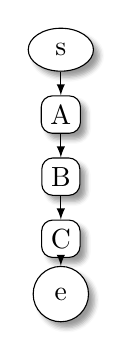
\begin{tikzpicture}[auto,
  node distance = 3mm,
  start chain = going below,
  start/.style = {ellipse,draw,text width= 1em,rounded corners,blur shadow,fill=white,
        on chain,align=center},
  box/.style = {draw,rounded corners,blur shadow,fill=white,
        on chain,align=center},
  stop/.style = {circle,minimum width=20pt,draw,blur shadow,fill=white,
        on chain,align=center}]
 \node[start] (b1)    {s};
 \node[box] (b2)    {A};
 \node[box] (b3)    {B};
 \node[box] (b4)    {C};
 \node[stop,below=1mm of b4] (b5)    {e};
 %\node[stop] (b5)    {e};
 \begin{scope}[rounded corners,-latex]
  \path
  (b1) edge (b2)
  (b2) edge (b3)
  (b3) edge (b4)
  (b4) edge (b5);
 \end{scope}
\end{tikzpicture}         
\caption{Sequence}
\label{tikz:sequence}
\end{subfigure}
\begin{subfigure}[h]{0.3\textwidth}
\centering

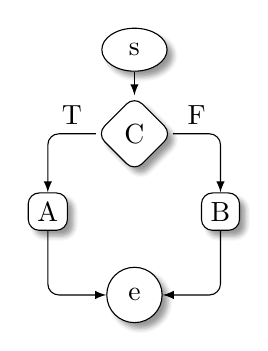
\begin{tikzpicture}[auto,
  node distance = 3mm,
  start chain = going below,
  start/.style = {ellipse,draw,text width= 1em,rounded corners,blur shadow,fill=white,
        on chain,align=center},
  box/.style = {draw,rounded corners,blur shadow,fill=white,
        on chain,align=center},
  cond/.style = {diamond,draw,rounded corners,blur shadow,fill=white,
        on chain,align=center},
  stop/.style = {circle,minimum width=20pt,draw,blur shadow,fill=white,
        on chain,align=center}
]
 \node[start] (b1)    {s};
 \node[cond] (b2)    {C};
 \node[box, below left=0.5cm and 0.6cm of b2] (b21) {A};
 \node[box, below right=0.5cm and 0.6cm of b2] (b22) {B};
 \node[stop,below=12mm of b2] (b3)    {e};
 \begin{scope}[rounded corners,-latex]
 \path
 (b1) edge (b2);
 \draw[-latex] (b2) -| node[pos=0.25,above] {T} (b21);
 \draw[-latex] (b2) -| node[pos=0.25,above] {F} (b22);
  \draw[-latex] (b21) |- (b3);
  \draw[-latex] (b22) |- (b3);
\end{scope}
\end{tikzpicture}
\caption{Condition}
\label{tikz:condition}
\end{subfigure}
\begin{subfigure}[h]{0.3\textwidth}
\centering
% \vspace{2.8cm}
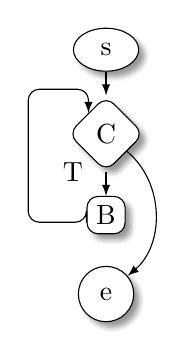
\begin{tikzpicture}[auto,
  node distance = 3mm,
  start chain = going below,
  start/.style = {ellipse,draw,text width= 1em,rounded corners,blur shadow,fill=white,
  on chain,align=center},
  box/.style = {draw,rounded corners,blur shadow,fill=white,
  on chain,align=center},
  cond/.style = {diamond,aspect=1,draw,rounded corners,blur shadow,fill=white,
  on chain,align=center},
  stop/.style = {circle,minimum width=20pt,draw,blur shadow,fill=white,
  on chain,align=center}]
 \node[start] (b1)    {s};      
 \node[cond] (b2)    {C};      
 \node[box] (b3)    {B};  
 %\node[stop] (b4)    {e};
 \node[stop,below=4mm of b3] (b4)    {e};
 \begin{scope}[rounded corners,-latex]
  \path (b2.-40) edge[bend left=50] (b4.40)
  (b1) edge node [midway,below, xshift=-12pt,yshift=-25pt] {T}(b2)
  (b2) edge (b3);
  \draw (b3.200) -- ++(0,0) -| ([xshift=-5mm]b2.west) |-
  ([yshift=3mm]b2.130) -- (b2.130);
  %\path (b3.230) edge[bend left=90] (b2);
 \end{scope}
\end{tikzpicture}
\caption{Iteration}
\label{tikz:iteration}
\end{subfigure}

\vspace{10pt}
\begin{subfigure}[h]{0.3\textwidth}
\begin{grammar}\centering
  <s> $\rightarrow$ <A> <B> <C>
\end{grammar}
\end{subfigure}
\begin{subfigure}[h]{0.3\textwidth}
\begin{grammar}\centering
    <s> $\rightarrow$ <C> \term{T} <A> | <C> \term{F} <B>
\end{grammar}
%\begin{grammar}\centering
%  <s> $\rightarrow$ <C> <IF>
 % 
 % <IF> $\rightarrow$ <A>
 % \alt <B>
%\end{grammar}
\end{subfigure}
\begin{subfigure}[h]{0.3\textwidth}
\begin{grammar}\centering
  <s> $\rightarrow$ <C> \term{T} <B> | <C> \term{F}
  %<L> $\rightarrow$ $\epsilon$\phantom{d a b c d f g}
  
\end{grammar}

\end{subfigure}

\caption{The basic control-flow structures}
\label{fig:cfg}
\end{figure*}
%\begin{figure*}
%  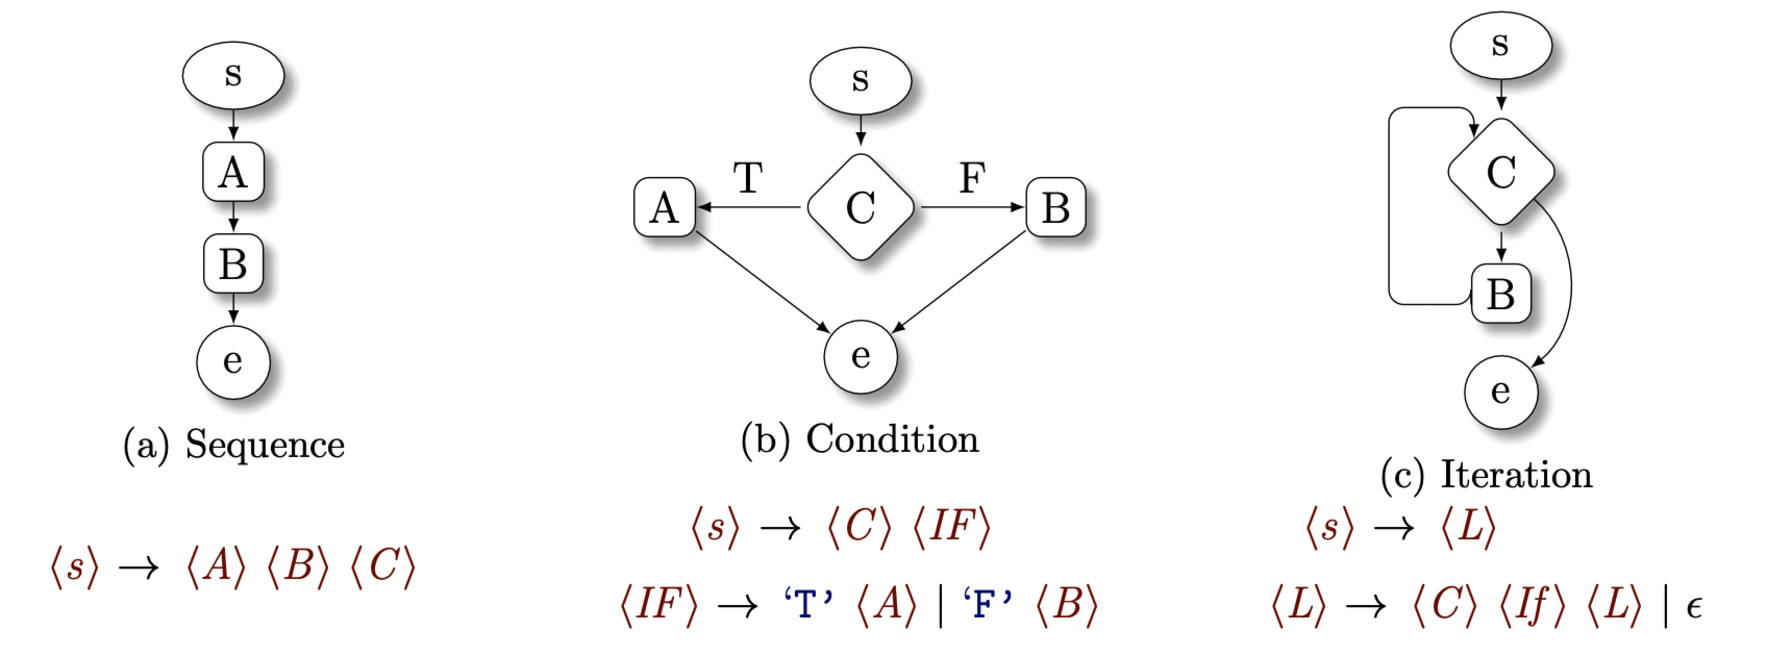
\includegraphics[width=\textwidth]{basiccfg.pdf}
%  \caption{Control flow to context-free grammar}
%  \label{fig:cfg}
%\end{figure*}

While synthetic benchmarks are a useful alternative, is it possible to use
real-world programs even if ground-truth (the maximum reachability) is not
known? A recent research on evaluating the reliability of biostatistics based
estimators for mutation analysis~\cite{Kuznetsov2024empirical} provides a
solution. The researchers point out that the \emph{sampling units} used in
species richness estimators should not have a significant effect on the final
estimate. In previous research on coverage estimation~\cite{liyanage2023reachable},
the sampling-unit used is the time interval. That is, the incidence data of
each 15-minutes bin was used as the sampling unit. Since the 15-minute interval
is arbitrary, it stands to reason that changing the timing granularity should
not impact the final estimate. Hence, we propose to evaluate the reliability of
maximum coverage estimators under varying granularity of sampling interval,
for the same fuzzing campaign duration.

% To be considered reliable, an estimator should yield consistent point estimates of maximum reachability across different sampling unit definitions, provided the total campaign length is held constant.

% Hence, in this paper, we propose to systematically investigate the reliability
% of incidence-based statistical estimators for maximum coverage.

\noindent{}\textbf{Contributions.}

\begin{itemize}
  \item \textbf{Synthetic benchmarks for evaluation:} We propose a novel
framework to generate synthetic program benchmarks that emulates real-world
programs, and use this to evaluate maximum reachability estimators.

  \item \textbf{Sampling-unit based evaluation of reliability} We will evaluate
    the reliability of maximum reachability estimators on 32 real-world programs
    by comparing the estimates under sampling units of diverse granularity.

  % We evaluate this framework on 32 real-world programs and demonstrate that certain estimators yield overlapping confidence intervals and reduced variance across different granularities—indicating estimator reliability.
    
% \item \textbf{Assessment of Stopping Criteria:} We re-examine previously proposed stopping criteria and evaluate their effectiveness in identifying when a statistical estimate may serve as a reliable upper bound on maximum reachability.

%\item\textcolor{red}{In this paper we propose a solution to the question of how to interpret the estimate from Chao on time based samples.}
\end{itemize}

The remainder of this paper is organized as follows. Section~\ref{sec:model} introduces the probabilistic model underlying fuzzing and the assumptions made in statistical reachability estimation. Section~\ref{sec:reachability} discusses current approaches to reachability estimation in fuzzing. Section~\ref{sec:method} presents our methodology for assessing the reliability of statistical estimators of maximum reachability. Section~\ref{sec:setup} details the experimental setup used to evaluate our approach. Finally, Section~\ref{sec:conclusion} concludes the paper and outlines directions for future research.

% ---- Model
\section{Preliminaries} \label{sec:model}

\subsection{Probabilistic Model for Fuzzing}

The STADS\footnote{STADS—Software Testing As Discovery of Species} framework~\cite{boehme2018stads,boehme2021residual,nguyen2022bedivfuzz,boehme2020boosting} formalizes
fuzzing as a statistical sampling process $\mathcal{F}$. Each test input is drawn with replacement from the program's input space $\pmb{\mathcal{D}}$. Assuming a sequence of $N$ independent and identically distributed (i.i.d.) random variables are drawn, we formally define the fuzzing campaign $\mathcal{F}$ as:

\begin{equation*}
    \mathcal{F}=\{X_n \mid X_n \in \pmb{\mathcal{D}}\}_{n=1}^N
\end{equation*}

The input space $\pmb{\mathcal{D}}$ consists of $S$ (potentially overlapping) subdomains $\{\mathcal{D}_i\}_{i=1}^S$, each representing a distinct \emph{coverage element}. An input $X_n \in \mathcal{F}$ is said to discover a \emph{new} coverage element $\mathcal{D}_i$ if $X_n \in \mathcal{D}_i$ and no earlier input $X_m \in \mathcal{F}$ for $m < n$ has been drawn from $\mathcal{D}_i$—that is, $\mathcal{D}_i$ is being encountered for the first time.


\subsection{Bernoulli Product Model}
Since each input in $\mathcal{F}$ may belong to one or more coverage elements, the STADS model represents coverage using \emph{sampling-unit-based incidence data}~\cite{colwell2012models,chao2017thirty}, where a sampling unit aggregates all inputs generated within a fixed time interval. The underlying probabilistic model for this representation is the \emph{Bernoulli product model}. Grouping inputs into sampling units is essential to reduce the overhead of tracking fine-grained coverage information for each individual input during fuzzing.

%This approach eliminates the need to record data for every individual test input in a fuzzing process that generates thousands of inputs per second. Instead, multiple inputs can be grouped into a \emph{sampling unit}.

For each sampling unit, the collected data indicates whether a coverage element
has been reached. Let $\pi_i$ denote the probability that a sampling unit covers
element $\mathcal{D}_i$, assuming $\pi_i$ remains constant across all randomly
selected sampling units.
In general, the sum of all $\pi_i$ values does \emph{not} equal unity.

During a fuzzing campaign, suppose we record $t$ sampling units. The incidence data forms an element$\times$sampling-unit incidence matrix ${W_{ij};i=1,2,\dots,S,j=1,2,\dots,t}$ with $S$ rows and $t$ columns, where $W_{ij} = 1$ if element $i$ is covered in sampling unit $j$, and $W_{ij} = 0$ otherwise.

The incidence frequency $Y_i$ represents the number of sampling units in which element $\mathcal{D}_i$ is covered; i.e., $Y_i=\sum_{j=1}^{t}W_{ij}$. A coverage element $\mathcal{D}_i$ that has not been covered by any sampling unit will have an incidence frequency of zero; i.e., $Y_i=0$.

Given the set of detection probabilities $(\pi_1,\pi_2,\dots,\pi_S)$, we assume each element $W_{ij}$ in the incidence matrix follows a Bernoulli distribution with probability $\pi_i$. The probability distribution for the incidence matrix is:

\begin{equation}
    \begin{split}
        P(W_{ij}=w_{ij};i=1,2,\dots,S,j=1,2,\dots,t) \\
        = \prod_{j=1}^{t}\prod_{i=1}^{S}\pi_i^{w_{ij}}(1-\pi_i)^{1-w_{ij}} \\
        = \prod_{i=1}^{S}\pi_i^{y_i}(1-\pi_i)^{t-y_i}.
    \end{split}
\end{equation}

The marginal distribution for the incidence-based frequency $Y_i$ for the $i$-th coverage element follows a binomial distribution characterized by $t$ and the detection probability $\pi_i$:

\begin{equation}
    P(Y_i=y_i) = \binom{t}{y_i}\pi_i^{y_i}(1-\pi_i)^{t-y_i}, \qquad i=1,2,\dots,S.
\end{equation}

Denote the incidence frequency counts by $(f_0, f_1, \dots, f_t)$, where $f_k$ is the number of elements covered in exactly $k$ sampling units in the data, $k=0,1,\dots,t$. Here, $f_1$ represents the number of \emph{singleton} elements (those that are covered in only one sampling unit), and $f_2$ represents the number of \emph{doubleton} elements (those that are covered in exactly two sampling units). The unobservable zero frequency count $f_0$ denotes the number of coverage elements that are not covered by any of the $t$ sampling units. Then, the number of covered elements in the current campaign is $S(t)=\sum_{i>0}f_i$, and $S(t)+f_0=S$.

%During a fuzzing campaign where we generate enormous amount of test inputs per unit time (at least thousands of inputs within seconds), it is not quite not practical to save the outcome for each input (i.e. the species $\mathcal{D}_i$ that our $X_n$ belongs to) in our data storage. Yet, it is a common practice to write such data at regular intervals. For instance, in our experimentation of 7-day fuzzing campaigns, we record incidence data once in every 15 minutes. Statistically, we can consider all the inputs generated between two consecutive recording instances as a sample of inputs and we indicate the detection/non-detection of species in this sample as a record. 
%

%Below we explain the probabilistic model for our fuzzing data. 
%
%\subsection{Probabilistic Model for Sampling-Unit-Based Data} \label{sec:probmodel}
%
%Assuming that the fuzzer's search space contains $S$ species, indexed by ${1,2,\dots,S}$. Without loss of generality, assume we have sampled $t$ sampling units, indexed by $1,2,\dots,t$, where each sampling unit represents a set of test inputs generated during a certain period of the ongoing fuzzing campaign. A species could be any choice of a program behaviour such as bugs or coverage elements like program paths, branches, or functions. It is assumed that these sampling units are randomly and independently sampled.


% ---- End Model
% --- Estimation
\subsection{Reachability Estimation in Fuzzing}
\label{sec:reachability}

\noindent\textbf{Estimators:} We build on prior work by continuing to use all state-of-the-art bio-statistical estimators for fuzzing effectiveness under the Bernoulli product model, as established in~\cite{liyanage2023reachable}. Additionally, inspired by recent studies on estimator performance for killable mutant prediction~\cite{Kuznetsov2024empirical}, we incorporate further estimators—including \emph{bootstrap}~\cite{smith1984nonparametric}, \emph{Zelterman}~\cite{bohning2010some}, and others previously unused in fuzzing—within our modeling framework.
\vspace{1mm}

\noindent\textbf{Ground Truth:} A fundamental challenge in evaluating estimators of fuzzing effectiveness lies in the absence of an absolute ground truth. 

%With the introduction of the STADS statistical framework and the growing adoption of fuzzing, understanding a fuzzer's detection capacity has become increasingly important. As a result, statistical techniques for estimating maximum reachability $\hat{S}$ have gained prominence \cite{boehme2018stads,liyanage2023reachable,boehme2019assurances}. Most estimators of $\hat{S}$ that conform to the probabilistic model in \autoref{sec:model} are introduced to fuzzing from the well-established field of ecological bio-statistics. However, challenges affecting the accuracy and precision of these estimates have been discussed both in the original STADS framework \cite{boehme2018stads} and in more recent evaluations \cite{liyanage2023reachable} of estimator performance. We discuss two critical challenges in more detail that we believe have a significant impact on reachability estimation and its evaluation in fuzzing.

%\subsection{Adaptive bias}
%A key statistical challenge in greybox fuzzing is \emph{adaptive bias}: as coverage-increasing inputs are added as new seeds, the distribution $\pi_i$ for $i: 1 \leq i \leq S$ evolves throughout the fuzzing campaign \cite{liyanage2021security}. A fundamental assumption of the Bernoulli Product model—common in statistics and machine learning—is that samples are independent and identically distributed (\emph{iid}), meaning the distribution of detection probabilities remains unchanged over time.  

%This assumption holds in blackbox fuzzing campaigns where no new seeds are added to the seed corpus while the fuzzer is running. However, in greybox fuzzing, which is the predominant fuzzing technique today, the outcome of one sample influences subsequent samples, violating the independence assumption \cite{boehme2020boosting,boehme2018stads,liyanage2021security}. Consequently, applying existing statistical estimators to greybox fuzzing leads to \emph{adaptive bias}, where estimates systematically over- or under-estimate the true value in greybox campaigns.

%Therefore, developing novel estimation strategies that correct adaptive bias in statistical estimation of key performance parameters is crucial for assessing greybox fuzzing progress and predicting its future trajectory. Recent advancements have introduced techniques that mitigate adaptive bias to estimate \emph{residual risk} \cite{boehme2021residual} and to extrapolate \emph{coverage rate} \cite{liyanage2024extrapolating} in greybox fuzzing. However, state-of-the-art reachability estimators continue to be affected by adaptive bias.


\subsection{Challenge of Establishing Ground Truth for Evaluation}

As with other software testing techniques, fuzzing aims to progressively explore diverse program behaviors—such as increasing code coverage or triggering distinct faults—over time. However, a fundamental challenge in evaluating the effectiveness of a fuzzing campaign lies in the absence of an absolute ground truth. Specifically, we can never be certain that all reachable program behaviors have been exercised, regardless of how long the fuzzer runs \cite{dijkstra2002ewd}. There always exists a non-zero probability that previously undiscovered behaviors may emerge as new test inputs are generated \cite{boehme2021residual}.

Despite this inherent uncertainty, the effectiveness of a fuzzing approach is often evaluated based on its maximum observed reachability within a fixed time or resource budget. For example, widely used benchmarks such as Fuzzbench \cite{metzman2021fuzzbench} and Magma \cite{hazimeh2020magma} assess fuzzers by measuring the coverage achieved after executing for a predetermined duration (e.g., 24 hours in the case of Fuzzbench). However, such evaluations can be misleading in scenarios where novel program behaviors are discovered beyond the allotted time window. This limitation underscores the need for more conclusive and robust quantitative techniques to assess fuzzing effectiveness—particularly methods grounded in data-driven estimation of maximum reachability. Still, establishing the ground truth remains a cornerstone for reliably evaluating such quantitative reachability measures.

\subsection{Existing Methods in Approximating Ground-Truth for Maximum Reachability}

Even though achieving a 100\% guarantee of exhausting all possible program behaviors is inherently unattainable, the longer a fuzzing campaign proceeds without encountering new behaviors, the lower the probability of discovering additional ones becomes. This diminishing discovery rate, in turn, increases our confidence in treating the current state as an empirical approximation of the ground truth for maximum reachability. However, recent empirical evidence based on extensive 7-day AFL++ \cite{fioraldi2020AFL++} fuzzing campaigns across 32 real-world C programs demonstrates that reaching a true asymptote in coverage is often elusive in practice \cite{liyanage2023reachable}. While coverage curves may appear to saturate when plotted on a linear scale, this effect is far less discernible on a logarithmic scale—suggesting that new behaviors continue to emerge at a slow but non-negligible rate. This observation further complicates the task of defining and approximating ground truth in fuzzing evaluation. Moreover, the same study highlights the limitations of using static analysis for estimating maximum reachable coverage, revealing both under- and over-approximation in practice. 

To address this challenge, the current fuzzing literature proposes state-of-the-art strategies to approximate ground-truth reachability, particularly for evaluating statistical estimators of maximum reachability:

\begin{enumerate}
    \item \textbf{Using small-scale programs as subjects:} When the subject program is relatively small and contains only a limited number of distinct reachable behaviors, fuzzers are more likely to achieve saturation within a feasible time frame. This makes such programs suitable proxies for maximum reachability estimator evaluations with ground-truth.
    
    \item \textbf{Bootstrapping from campaign data:} After executing a fuzzer for a sufficiently long period—ideally until the coverage or bug discovery curve exhibits signs of plateauing—bootstrap resampling can be applied to the observed data. The key intuition is that the relationship between the empirical distribution of discovered behaviors and the underlying theoretical population mirrors the relationship between bootstrap samples and the empirical distribution. This method enables statistical approximation of ground-truth reachability without requiring absolute exhaustiveness.
\end{enumerate}

\subsection{Drawbacks of Existing Ground-Truth Approaches}

Despite efforts to approximate ground truth in fuzzing evaluation, existing methods, particularly those relying on small-scale programs, have significant limitations. While small programs enable faster saturation of program behaviors, they fail to reflect the complexity and diversity of real-world systems, which often exhibit a highly skewed distribution of behaviors—similar to ecological environments with a few abundant behaviors and many rare ones. In contrast, smaller programs tend to have a less skewed distribution of species, leading to an overestimation of fuzzing estimators’ accuracy. This discrepancy results in misleading conclusions when performance estimators derived from small-scale programs are applied to larger, more complex systems, where the species distribution is less predictable. Consequently, the primary drawback of using small-scale programs for ground-truth approximation is the risk of overstating the effectiveness of fuzzing approaches when applied to real-world software.

In the case of bootstrapping, the core assumption—that the empirical distribution obtained from a fuzzing campaign reasonably approximates the true underlying distribution of all possible program behaviors—fails to satisfy when the campaign has not yet thoroughly explored critical regions of the codebase or when input generation is inherently biased. This assumption further relies on the expectation that the future trajectory of behavior discovery will not significantly deviate from its current trend, implying that species accumulation will smoothly approach saturation. However, without additional quantitative evidence to support the stability of this trajectory—such as statistical indicators of diminishing returns or convergence metrics—such assumptions remain speculative. In the absence of such validation, bootstrapped estimates may result in substantial over- or under-estimations of maximum reachability, ultimately undermining the reliability of fuzzing effectiveness evaluations.  

These limitations highlight the need for more robust, scalable, and accurate methods of defining and approximating ground truth in fuzzing evaluation, particularly as programs grow in size and complexity.

% --- End Estimation
% --- Methodology
\section{Methodology} \label{sec:method}
\begin{figure*} %{r}{7cm} %[12]
  \centering
\begin{subfigure}[h]{0.45\textwidth} %22 min
  \centering
%\begin{subfigure}
\lstset{numbers=left,xleftmargin=2em, numberstyle=\color{lightgray}
} %frame=single,framexleftmargin=1.5em}
\begin{lstlisting}[style=Python, escapechar=|,numbersep=2pt]
def bsearch(x, v, n):
  low, high = 0, n-1
  while low <= high:
    mid=(low+high)/2
    if x < v[mid]:
      high=mid-1
    else:
      if x > v[mid]:
        low=mid+1
      else:
        return mid
  return None
\end{lstlisting}
\caption{\<bsearch> program}
\label{fig:bsearch1}
\end{subfigure}
\begin{subfigure}[h]{0.45\textwidth}   %28 min
  \centering
\begin{grammar}%\centering
  <bsearch> $\rightarrow$ \term{l.2} <while.3> \term{l.12}

  <while.3> $\rightarrow$ \term{l.3}
   \alt \term{l.3} \term{l.4} \term{l.5} <if.5> <while.3>

  <if.5>  $\rightarrow$  \term{T} \term{l.6}
   \alt \term{F} \term{l.8} <if.8>

  <if.8> $\rightarrow$ \term{T} \term{l.9}
   \alt \term{F} \term{l.11}
\end{grammar}
\caption{\<bsearch> control-flow grammar}
\label{fig:bsearch3}
\end{subfigure}
\caption{Extracting the context-free grammar for \<bsearch>}
\label{fig:bsearch}
\end{figure*}
We next describe our proposed methodology for overcoming the limitations discussed in \Cref{sec:reachability}.
\subsection{Evaluating Estimators of \texorpdfstring{$\hat{S}$}{S-hat} Against Accurate Ground Truth}
To overcome the problem due to non-availability of complex programs with available
maximum coverage, we propose a novel methodology.

We note that any structured program can be translated into a simpler program
such that it contains only the following elements:
(1) sequence of statements
(2) if-then-else conditionals
(3) \<while> loops
(4) procedure calls.
Next, given such a simplified form and its control-flow,
we can leverage the following rules to convert the control-flow to the context-free grammar~(\Cref{fig:cfg}).
That is, (1) for any given \<while C: L> loop, with a boolean conditional \<C>,
it can be translated to an equivalent grammar rule
%\begin{grammar}
  \mbox{\nonterm{L} \expandsto \nonterm{C} \nonterm{L} $|$ \nonterm{C}}
%\end{grammar}
(2) for any conditional \<if C: B else: D>, translate to
  \mbox{\nonterm{IF} \expandsto \nonterm{C} \term{T} \nonterm{B}  $|$ \nonterm{C} \term{F} \nonterm{D}}
(3) procedure definitions such as \<def P(): B \ldots> translate to a nonterminal symbol with the same
name: \mbox{\nonterm{P} \expandsto \nonterm{B}}, and sequence of statements are simply captured
directly with corresponding tokens.
The details are given in \Cref{fig:cfg}.

Given that \emph{any structured program} can thus be translated into a
context-free grammar, the space of possible context-free grammars are also
the space of control-flows of possible programs. Hence, to evaluate how
an estimator performs on the reachability of all possible programs, it is
sufficient to generate a statistically significant number of complex
context-free programs that represent control-flows, and translate them back
to programs. This raises a question. How can we translate these control-flows
to equivalent programs with the same control flow.

Fortunately, there's a simple answer. Given any non-left-recursive context-free
grammar, we can generate a recursive-descent parser using these rules:
(1) Each nonterminal \nonterm{E} becomes a function \<def parse\_E>.
(2) Each production rule is implemented in that function.
(3) Lookahead tokens guide which rule to apply.
(4) Linear recursion can be replaced with a \<while> loop.
%Fortunately, there is an easy naswer. Given any non left-recursive context-free
%grammar, we can generate a recursive-descent parser by using the following rules:
%(1) Any nonterminal symbol in the grammar is turned into a procedure in the parser.
%(2) Each production rule is also turned into a procedure in the parser.
%(3) The particular rule to be used to parse is based on the \emph{lookahead}
%corresponding to each rule that matches the current symbol.
%(4) Any linear recursive nonterminal-rule combination is converted into a \texttt{while} loop.

Following in this fashion, we get a parser that directly corresponds to the context-free
grammar. For example, given the grammar 
\nonterm{E}\expandsto \nonterm{D} \nonterm{Es};
\nonterm{Es}\expandsto \term{+}\nonterm{D}\nonterm{Es}$|$ $\epsilon$, we can translate
this to:
\begin{lstlisting}[style=Python, escapechar=|,numbersep=2pt]
def parse_E():
  parse_D()

  while lookahead() == '+':
    consume('+')
    parse_D()
  return node

def parse_D():
  token = lookahead()
  if token and isdigit(token):
    consume(token)
  else:
    raise Error()
\end{lstlisting}
which has similar control-flow as a program from which such a grammar may have
been obtained.

While generating context-free grammars, we have several mechanisms to
precisely control the complexity. These include:
(1) The number of nonterminal symbols in the grammar
(2) The number of production rules
(3) The number of alphabets in the language
(4) The amount of direct and indirect recursion
(5) The length of individual rules
(6) The VC dimension of the language.
These parameters allow us to generate large scale parser programs at will with
complex control-flows. We can additionally increase the difficulty level by
adding extra constraints to the generated parser such
as context-sensitivity.

\noindent\textbf{Scalability and Applicability:} This methodology is designed to generate large-scale C parsers that consist of thousands of lines of code and complex control-flow.

\subsection{Assessing Reliability \texorpdfstring{$\hat{S}$}{S-hat} Estimators Without Ground truth}
To overcome any limitation that may exist due to the synthetic nature of our
previously proposed benchmark, we propose a second criterion that can be applied
to real-world benchmarks without relying on availability of ground truth.

Our approach is inspired by the previous research on equivalent mutant
estimation~\cite{Kuznetsov2024empirical}, which suggests that varying
sample-units can be leveraged to evaluate the reliability of estimators.
The idea is that, while incidence-based statistical estimators of
fuzzing effectiveness may be sensitive to the sampling unit size ($r$),
a reliable estimator should produce overlapping point estimates for $S$—with
varying variance but consistent expectation when evaluated over equal-length
campaigns.

We propose to evaluate whether estimators of maximum reachability $S$ yield
consistent point estimates with overlapping confidence intervals, while allowing
for differences in estimation accuracy (i.e., variability) across fuzzing
campaigns with different sampling unit definitions $r$.


% TODO: This should be in the previous section. Not here.
% Prior empirical research on estimating maximum reachable coverage in fuzzing
% campaigns—under the Bernoulli product model—has shown that statistical
% estimators systematically underestimate true reachability until near
% saturation, a phenomenon termed \emph{false peaks}~\cite{liyanage2023reachable}.
% This negative bias is largely inevitable in early stages due to the
% insufficiency of fuzzing data and the heterogeneous species diversity,
% which limits accurate approximation of the species distribution.
% 
% Prior research~\cite{liyanage2023reachable} empirically investigated this
% phenomenon, and suggests that estimators become reliable when the
% count of doubletons equals or exheeds singletons.

%  These limitations prompt a critical question: \emph{How can we ensure that statistical estimators provide reliable approximations of maximum reachability $S$ in fuzzing campaigns?}
% 
% \result{\textbf{Intuition:} While incidence-based statistical estimators of fuzzing effectiveness are sensitive to the sampling unit size ($r$), a reliable estimator should produce overlapping point estimates for $S$—with varying variance but consistent expectation—when evaluated over equal-length campaigns.}
% 
% The incidence frequency counts—particularly singletons ($f_1$) and doubletons ($f_2$)—are sensitive to the granularity of the sampling unit ($r$). Using individual inputs ($r=1$) yields the most fine-grained data, while aggregating inputs (e.g., over time intervals) reduces resolution. Aggregation tends to decrease $f_1$ and increase higher-frequency counts, as rare elements may co-occur within a unit. Since estimators like Chao2 depend directly on $f_1$ and $f_2$, the point estimate of species richness $\hat{S}$ may vary with changes in $r$, even under equal-length campaigns. Despite this sensitivity, the choice of $r$ is often arbitrary; for instance, \cite{liyanage2023reachable} adopts 15-minute intervals without justification.
% 
% However, since the maximum reachability $S$ is a finite quantity for any given fuzzing campaign, a reliable estimator should approximate it within reasonable error bounds—despite variability in incidence frequencies introduced by changes in the sampling unit definition—provided that the estimation is performed at the same time point since the campaign's start. Leveraging this property, we evaluate whether estimators of maximum reachability $S$ yield consistent point estimates with overlapping confidence intervals, while allowing for differences in estimation accuracy (i.e., variability) across fuzzing campaigns with different sampling unit definitions $r$.

% \textcolor{red}{Stopping Criterion Evaluation:
% Evaluate the stopping criterion in checking the reliability of reachability estimators. (Applicable beyond f1 <f2) By evaluating f1 actually becomes an upper bound to f0.
%}
% --- End Methodology


\section{Experimental Setup} \label{sec:setup}

\subsection{Research Questions}

This study addresses the following research questions:

\begin{itemize}
    \item \textbf{RQ1:} How accurately do statistical estimators of maximum reachability approximate the ground truth obtained using our proposed ensemble measurement approach?
    
    \item \textbf{RQ2:} How does the performance of estimators based on our proposed ground truths compare to their performance using ground truths from prior studies?
    
    \item \textbf{RQ3:} To what extent are the estimates of maximum reachability $S$ sensitive to changes in the sampling unit size $r$?
\end{itemize}

\subsection{Fuzzers and Subject Programs}

For our experiments, we use AFL++ \cite{fioraldi2020AFL++}, a widely recognized state-of-the-art greybox fuzzer known for its performance and extensive adoption in recent research, particularly in reachability estimation studies. Using the same fuzzer as prior work enables direct and fair comparisons when evaluating estimator performance (RQ2).

We select a diverse set of real-world C programs from the FuzzBench platform \cite{metzman2021fuzzbench}, which provides a standardized fuzzing benchmarking environment. To ensure comparability with earlier studies (specifically for RQ2), we include all subject programs used in \cite{liyanage2023reachable}, along with several additional targets that are compatible with AFL++ and suitable for large-scale fuzzing.


\section{Related Work}

Reachable program behaviors (e.g. code coverage and discovered bugs) determine the \emph{effectiveness} of a software testing process. For non-trivial programs, exhaustively exercising all possible behaviors is infeasible. Consequently, testing is often viewed as a means to demonstrate the presence of bugs, but not their absence~\cite{dijkstra2022reliability}. Despite this limitation, substantial effort has been directed toward increasing maximum reachability to enhance software security and reliability. Nevertheless, determining reachability remains a fundamental challenge in software testing. In fact, an efficient and precise determination of reachable code would effectively resolve the software verification problem~\cite{liyanage2023reachable}. 

Efforts to approximate reachability quantitatively have gained traction in the security domain, despite inherent difficulties. Empirical studies indicate that establishing the reachability of certain code regions is particularly challenging in large, complex code bases, using both static and dynamic analysis techniques~\cite{latoza2010developers}. Static analysis methods, such as symbolic execution, often suffer from over- or under-approximation when estimating reachable coverage~\cite{liyanage2023reachable,aniche2015why}. For instance, Nikoli\'{c} and Spoto~\cite{nikolic2013reachability} proposed approximating the reachability of program variables as a new abstract domain for static analysis. While their approach yields over-approximations, authors argue that it can be conservatively applied to identify unreachable code. Similarly, Mikol\'{a}\v{s} et al.~\cite{janota2007reachability} leveraged annotated code to define unreachability conditions and proposed an efficient algorithm for detecting unreachable code.

To assess reachability or unreachability in dynamic analysis, both constraint-solving techniques such as SMT\footnote{SMT—Satisfiability Modulo Theory} and data-driven estimation methods have been explored. Naus et al.~\cite{naus2023low} proposed a technique for automatically generating preconditions to trigger specific post-conditions (e.g., bugs) using low-level code analysis. Similarly, Liew et al.~\cite{liew2019just} demonstrated how to encode SMT formulas within coverage-guided fuzzers to discover inputs that reach targeted program locations. In contrast, statistical approaches directly attempt to estimate the test effectiveness (aka maximum reachability) through observed behaviors. The pioneering STADS framework~\cite{boehme2018stads} introduced a suite of bio-statistical estimators by modeling fuzzing as a statistical sampling process. A recent evaluation of these estimators highlighted key challenges associated with reachability estimation~\cite{liyanage2023reachable}. When applied to estimate the number of killable mutants in mutation analysis, Kuznetsov et al.~\cite{Kuznetsov2024empirical} empirically demonstrated the unreliability of STADS estimators due to variations in sampling unit definitions. This finding, together with other recent studies, underscores the need for \emph{structure-aware} estimators that incorporate internal program structure, as opposed to structure-agnostic alternatives~\cite{lee2023statistical}.


\section{Conclusion}
\label{sec:conclusion}
In this report, we propose to assess the reliability of species estimators when
they are used for estimating reachable coverage. We propose to do that both by
providing a synthetic benchmark with labeled ground truth, and also by
using a separate means of checking the reliability of estimators by varying
the sampling units used.

%\section{Authors and Affiliations}


\bibliographystyle{IEEEtran}
\bibliography{icsme-registered.bib}


%\section{Acknowledgments}

%% If your work has an appendix, this is the place to put it.
%\appendix

\end{document}
\endinput
%%
%% End of file `sample-manuscript.tex'.
